\label{Intro.}
Water, being ``at the centre of the planetary drama of the Anthropocene'' \cite{gleesonIlluminatingwatercycle2020}, is essential not only for earth system processes but also in supporting development and human well-being.
As an integral part of a proposed earth system governance framework, water governance requires a deep understanding of changes in the complex relationships between humans and water
\cite{dibaldassarreSociohydrologyScientificChallenges2019,biermannNavigatingAnthropoceneImproving2012,steffenemergenceevolutionEarth2020}.
Human activities stemming from our reliance on the water have profoundly modified the natural water cycle, resulting in rivers dominated by a hybrid of social and natural tendencies
\cite{gleesonIlluminatingwatercycle2020,sivapalanSociohydrologynewscience2012,qinTheoreticalframeworkdualistic2014,abbottwatercycleAnthropocene2019,leviaHomogenizationterrestrialwater2020}.
Facing this transition, many big river basins worldwide (which are hot spots of civilization and economic growth) are urgently in need of successful water governance for sustainability
\cite{bestAnthropogenicstressesworld2019,falkenmarkUnderstandingwaterresilience2019,dibaldassarreSociohydrologyScientificChallenges2019}.

Water governance refers to the political, social, economic, and administrative systems that influence the use and management of water %! citation.
For populated large river basins, missing governance means missing sustainability, and a first important step in understanding the transitions with successful water governance is identifying the different regimes.
\cite{undpwatergovernancefacilityWaterGovernanceIssue}.
Regimes of water governance maintained by concreted intertwine within human-water systems (such as management, institutions, and exploitations), as a stable state in structures and functions
\cite{carpenterEarlyWarningsRegime2011,rochaCascadingregimeshifts2018, gregrCascadingsocialecologicalcosts2020}.
Therefore, regime shifts sometimes lead to new water governance challenges as both signals and consequences of substantive changes in human-water systems.
The lack of a comprehensive but straightforward approach to identifying changes in water governance regimes challenges sustainability, and filling this gap can well align human and water systems (Figure~\ref{fig:framework}).

Governance is essentially about ``who gets what, when and how''. The United Nations Development Programme (UNDP) thus suggested that three key dimensions of water use are decided by the water governance directly: ``When and what water to use?'' (stress), ``How does water provides different services to well-beings?'' (purpose), and ``Who can use water equally and efficiently?'' (allocation)
\cite{undpwatergovernancefacilityWaterGovernanceIssue, mariajacobsonUserguideassessing2013, kjellenWatergovernanceperspective2015}. %! UNDP year
First, water stress depends not only on climate (with increasing scarcity and uncertainty in many regions) but also on the increasingly insatiable demands from economic activities such as irrigation and industry; water storage can resolve some but not all of these issues
\cite{greveGlobalassessmentwater2018,wadaHumanwaterinterface2017,qinFlexibilityintensityglobal2019}.
Second, the purpose of how water services human well-being is to consider trade-offs between consumptive uses (e.g., drinking and food production) and non-consumptive uses (e.g., energy production)
\cite{liuWaterscarcityassessments2017,florkeWatercompetitioncities2018,kleemannQuantifyinginterregionalflows2020}.
Third, the allocation of water across the whole basin is not only decided by regionally socio-economic and environmental context but also influenced by systematically regulating
\cite{roobavannanRoleSectoralTransformation2017,speedBasinwaterallocation2013}.
Despite regime shifts in water governance related to substantive changes in any of the three dimensions, separately considering their intertwines within human-water systems can lead to holistic failure in governing water.

The Yellow River Basin (YRB), the fifth-largest river in the world, was most in need of integrated water governance because drastically anthropogenic intervention led to intense governance challenges in sustainability (see \textit{Appendix} Methods S1 and Figure S1 for details).
Since the 1960s, the implementation of conservation measures, regulation reservoirs, and levee constructions have contained the governance issues troubled by thousands of years of high sediment loads
\cite{wangReducedsedimenttransport2016,wuEvolutioneffectssocialecological2020}.
However, decreased streamflows and water over-use then led to depletions of the over-burdened river, creating new challenges and new governance practices, including water use regulation and water transfer across basins
\cite{xiaDevelopmentWaterAllocation2012}.
Today, it is still impossible to completely solve water stress, trade-offs between ecosystem services, or lopsided development in different regions in the YRB; -``who gets water, when and how‘’ is always an open question for sustainable development
\cite{wangYellowRiverwater2019,wohlfartSocialecologicalchallengesYellow2016}.
Confronting governance challenges induced by environmental, economic, social, and political factors, numerous governance practices have led the YRB to be among the most drastically-governing large river basins worldwide
Identifying regime shifts in water governance within the YRB can thus provide crucial insights into rapidly-changing big river basins and how governance may respond to meeting challenges to their sustainability.

% 这里我们整合了三个方向,提出了描绘流域人水关系的指数
Here, we use the three core dimensions (stress, purpose and allocation) and corresponding indicators of water governance to develop an Integrated Water Governance Index (IWGI) that can detect and describe changes in water governance at a basin-scale (see Figure~\ref{fig:framework} and methods).
% 使用案例研究
Then, by applying the index to a typical rapid-changing big river basin (the YRB), we show how to analyze the complicated water governance regimes in a comprehensive but straightforward way.
Following synthetic analyses of the changes in water demand, supply, economic outcomes, and institutions, we interpret the leading causes of the regime shifts.
% 最后总结出一般性框架
Finally, we propose a general regime transition schema as a practical guideline for a coordinated approach to exploring the challenges faced by big river basin governance.

\begin{figure*}[!ht]
	\centering
	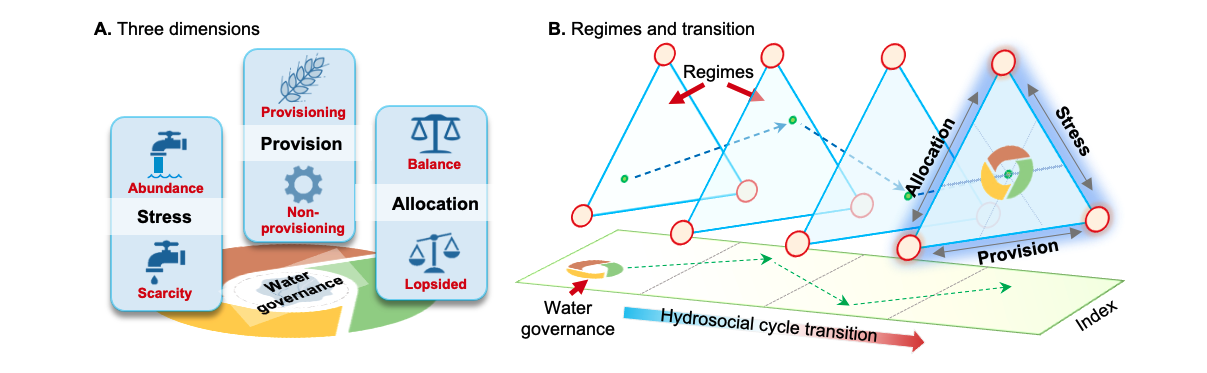
\includegraphics[width=0.9\textwidth]{main/framework.png}
	\caption{
		Identifying the water governance regimes in transitions of a hydrosocial cycle.
		\textbf{A.} Water governance has three key dimensions (stress, purpose and allocation), each of which has two potential directions (denoted in red) when changing. (1) ``stress'' of water shifts between scarcity and abundance; (2) weighting ``purpose'' of water between consumptive services or non-consumptive uses; (3) ``allocation'' changes between balanced or lopsided.
		\textbf{B.} Along with a transition in hydrosocial water cycle, water governance shifts in line with the three dimensions. Combining corresponding indicators, an abrupt change of the IWGI thus indicates a regime shift in water governance.
		% \cite{steffenTrajectoriesEarthSystem2018,abbottwatercycleAnthropocene2019,leviaHomogenizationterrestrialwater2020}.
	}
	\label{fig:framework}
\end{figure*}
